\documentclass[10pt]{article}
\usepackage{tmlr}
%%%%% NEW MATH DEFINITIONS %%%%%

\usepackage{amsmath,amsfonts,bm}

% Mark sections of captions for referring to divisions of figures
\newcommand{\figleft}{{\em (Left)}}
\newcommand{\figcenter}{{\em (Center)}}
\newcommand{\figright}{{\em (Right)}}
\newcommand{\figtop}{{\em (Top)}}
\newcommand{\figbottom}{{\em (Bottom)}}
\newcommand{\captiona}{{\em (a)}}
\newcommand{\captionb}{{\em (b)}}
\newcommand{\captionc}{{\em (c)}}
\newcommand{\captiond}{{\em (d)}}

% Highlight a newly defined term
\newcommand{\newterm}[1]{{\bf #1}}


% Figure reference, lower-case.
\def\figref#1{figure~\ref{#1}}
% Figure reference, capital. For start of sentence
\def\Figref#1{Figure~\ref{#1}}
\def\twofigref#1#2{figures \ref{#1} and \ref{#2}}
\def\quadfigref#1#2#3#4{figures \ref{#1}, \ref{#2}, \ref{#3} and \ref{#4}}
% Section reference, lower-case.
\def\secref#1{section~\ref{#1}}
% Section reference, capital.
\def\Secref#1{Section~\ref{#1}}
% Reference to two sections.
\def\twosecrefs#1#2{sections \ref{#1} and \ref{#2}}
% Reference to three sections.
\def\secrefs#1#2#3{sections \ref{#1}, \ref{#2} and \ref{#3}}
% Reference to an equation, lower-case.
\def\eqref#1{equation~\ref{#1}}
% Reference to an equation, upper case
\def\Eqref#1{Equation~\ref{#1}}
% A raw reference to an equation---avoid using if possible
\def\plaineqref#1{\ref{#1}}
% Reference to a chapter, lower-case.
\def\chapref#1{chapter~\ref{#1}}
% Reference to an equation, upper case.
\def\Chapref#1{Chapter~\ref{#1}}
% Reference to a range of chapters
\def\rangechapref#1#2{chapters\ref{#1}--\ref{#2}}
% Reference to an algorithm, lower-case.
\def\algref#1{algorithm~\ref{#1}}
% Reference to an algorithm, upper case.
\def\Algref#1{Algorithm~\ref{#1}}
\def\twoalgref#1#2{algorithms \ref{#1} and \ref{#2}}
\def\Twoalgref#1#2{Algorithms \ref{#1} and \ref{#2}}
% Reference to a part, lower case
\def\partref#1{part~\ref{#1}}
% Reference to a part, upper case
\def\Partref#1{Part~\ref{#1}}
\def\twopartref#1#2{parts \ref{#1} and \ref{#2}}

\def\ceil#1{\lceil #1 \rceil}
\def\floor#1{\lfloor #1 \rfloor}
\def\1{\bm{1}}
\newcommand{\train}{\mathcal{D}}
\newcommand{\valid}{\mathcal{D_{\mathrm{valid}}}}
\newcommand{\test}{\mathcal{D_{\mathrm{test}}}}

\def\eps{{\epsilon}}


% Random variables
\def\reta{{\textnormal{$\eta$}}}
\def\ra{{\textnormal{a}}}
\def\rb{{\textnormal{b}}}
\def\rc{{\textnormal{c}}}
\def\rd{{\textnormal{d}}}
\def\re{{\textnormal{e}}}
\def\rf{{\textnormal{f}}}
\def\rg{{\textnormal{g}}}
\def\rh{{\textnormal{h}}}
\def\ri{{\textnormal{i}}}
\def\rj{{\textnormal{j}}}
\def\rk{{\textnormal{k}}}
\def\rl{{\textnormal{l}}}
% rm is already a command, just don't name any random variables m
\def\rn{{\textnormal{n}}}
\def\ro{{\textnormal{o}}}
\def\rp{{\textnormal{p}}}
\def\rq{{\textnormal{q}}}
\def\rr{{\textnormal{r}}}
\def\rs{{\textnormal{s}}}
\def\rt{{\textnormal{t}}}
\def\ru{{\textnormal{u}}}
\def\rv{{\textnormal{v}}}
\def\rw{{\textnormal{w}}}
\def\rx{{\textnormal{x}}}
\def\ry{{\textnormal{y}}}
\def\rz{{\textnormal{z}}}

% Random vectors
\def\rvepsilon{{\mathbf{\epsilon}}}
\def\rvtheta{{\mathbf{\theta}}}
\def\rva{{\mathbf{a}}}
\def\rvb{{\mathbf{b}}}
\def\rvc{{\mathbf{c}}}
\def\rvd{{\mathbf{d}}}
\def\rve{{\mathbf{e}}}
\def\rvf{{\mathbf{f}}}
\def\rvg{{\mathbf{g}}}
\def\rvh{{\mathbf{h}}}
\def\rvu{{\mathbf{i}}}
\def\rvj{{\mathbf{j}}}
\def\rvk{{\mathbf{k}}}
\def\rvl{{\mathbf{l}}}
\def\rvm{{\mathbf{m}}}
\def\rvn{{\mathbf{n}}}
\def\rvo{{\mathbf{o}}}
\def\rvp{{\mathbf{p}}}
\def\rvq{{\mathbf{q}}}
\def\rvr{{\mathbf{r}}}
\def\rvs{{\mathbf{s}}}
\def\rvt{{\mathbf{t}}}
\def\rvu{{\mathbf{u}}}
\def\rvv{{\mathbf{v}}}
\def\rvw{{\mathbf{w}}}
\def\rvx{{\mathbf{x}}}
\def\rvy{{\mathbf{y}}}
\def\rvz{{\mathbf{z}}}

% Elements of random vectors
\def\erva{{\textnormal{a}}}
\def\ervb{{\textnormal{b}}}
\def\ervc{{\textnormal{c}}}
\def\ervd{{\textnormal{d}}}
\def\erve{{\textnormal{e}}}
\def\ervf{{\textnormal{f}}}
\def\ervg{{\textnormal{g}}}
\def\ervh{{\textnormal{h}}}
\def\ervi{{\textnormal{i}}}
\def\ervj{{\textnormal{j}}}
\def\ervk{{\textnormal{k}}}
\def\ervl{{\textnormal{l}}}
\def\ervm{{\textnormal{m}}}
\def\ervn{{\textnormal{n}}}
\def\ervo{{\textnormal{o}}}
\def\ervp{{\textnormal{p}}}
\def\ervq{{\textnormal{q}}}
\def\ervr{{\textnormal{r}}}
\def\ervs{{\textnormal{s}}}
\def\ervt{{\textnormal{t}}}
\def\ervu{{\textnormal{u}}}
\def\ervv{{\textnormal{v}}}
\def\ervw{{\textnormal{w}}}
\def\ervx{{\textnormal{x}}}
\def\ervy{{\textnormal{y}}}
\def\ervz{{\textnormal{z}}}

% Random matrices
\def\rmA{{\mathbf{A}}}
\def\rmB{{\mathbf{B}}}
\def\rmC{{\mathbf{C}}}
\def\rmD{{\mathbf{D}}}
\def\rmE{{\mathbf{E}}}
\def\rmF{{\mathbf{F}}}
\def\rmG{{\mathbf{G}}}
\def\rmH{{\mathbf{H}}}
\def\rmI{{\mathbf{I}}}
\def\rmJ{{\mathbf{J}}}
\def\rmK{{\mathbf{K}}}
\def\rmL{{\mathbf{L}}}
\def\rmM{{\mathbf{M}}}
\def\rmN{{\mathbf{N}}}
\def\rmO{{\mathbf{O}}}
\def\rmP{{\mathbf{P}}}
\def\rmQ{{\mathbf{Q}}}
\def\rmR{{\mathbf{R}}}
\def\rmS{{\mathbf{S}}}
\def\rmT{{\mathbf{T}}}
\def\rmU{{\mathbf{U}}}
\def\rmV{{\mathbf{V}}}
\def\rmW{{\mathbf{W}}}
\def\rmX{{\mathbf{X}}}
\def\rmY{{\mathbf{Y}}}
\def\rmZ{{\mathbf{Z}}}

% Elements of random matrices
\def\ermA{{\textnormal{A}}}
\def\ermB{{\textnormal{B}}}
\def\ermC{{\textnormal{C}}}
\def\ermD{{\textnormal{D}}}
\def\ermE{{\textnormal{E}}}
\def\ermF{{\textnormal{F}}}
\def\ermG{{\textnormal{G}}}
\def\ermH{{\textnormal{H}}}
\def\ermI{{\textnormal{I}}}
\def\ermJ{{\textnormal{J}}}
\def\ermK{{\textnormal{K}}}
\def\ermL{{\textnormal{L}}}
\def\ermM{{\textnormal{M}}}
\def\ermN{{\textnormal{N}}}
\def\ermO{{\textnormal{O}}}
\def\ermP{{\textnormal{P}}}
\def\ermQ{{\textnormal{Q}}}
\def\ermR{{\textnormal{R}}}
\def\ermS{{\textnormal{S}}}
\def\ermT{{\textnormal{T}}}
\def\ermU{{\textnormal{U}}}
\def\ermV{{\textnormal{V}}}
\def\ermW{{\textnormal{W}}}
\def\ermX{{\textnormal{X}}}
\def\ermY{{\textnormal{Y}}}
\def\ermZ{{\textnormal{Z}}}

% Vectors
\def\vzero{{\bm{0}}}
\def\vone{{\bm{1}}}
\def\vmu{{\bm{\mu}}}
\def\vtheta{{\bm{\theta}}}
\def\va{{\bm{a}}}
\def\vb{{\bm{b}}}
\def\vc{{\bm{c}}}
\def\vd{{\bm{d}}}
\def\ve{{\bm{e}}}
\def\vf{{\bm{f}}}
\def\vg{{\bm{g}}}
\def\vh{{\bm{h}}}
\def\vi{{\bm{i}}}
\def\vj{{\bm{j}}}
\def\vk{{\bm{k}}}
\def\vl{{\bm{l}}}
\def\vm{{\bm{m}}}
\def\vn{{\bm{n}}}
\def\vo{{\bm{o}}}
\def\vp{{\bm{p}}}
\def\vq{{\bm{q}}}
\def\vr{{\bm{r}}}
\def\vs{{\bm{s}}}
\def\vt{{\bm{t}}}
\def\vu{{\bm{u}}}
\def\vv{{\bm{v}}}
\def\vw{{\bm{w}}}
\def\vx{{\bm{x}}}
\def\vy{{\bm{y}}}
\def\vz{{\bm{z}}}

% Elements of vectors
\def\evalpha{{\alpha}}
\def\evbeta{{\beta}}
\def\evepsilon{{\epsilon}}
\def\evlambda{{\lambda}}
\def\evomega{{\omega}}
\def\evmu{{\mu}}
\def\evpsi{{\psi}}
\def\evsigma{{\sigma}}
\def\evtheta{{\theta}}
\def\eva{{a}}
\def\evb{{b}}
\def\evc{{c}}
\def\evd{{d}}
\def\eve{{e}}
\def\evf{{f}}
\def\evg{{g}}
\def\evh{{h}}
\def\evi{{i}}
\def\evj{{j}}
\def\evk{{k}}
\def\evl{{l}}
\def\evm{{m}}
\def\evn{{n}}
\def\evo{{o}}
\def\evp{{p}}
\def\evq{{q}}
\def\evr{{r}}
\def\evs{{s}}
\def\evt{{t}}
\def\evu{{u}}
\def\evv{{v}}
\def\evw{{w}}
\def\evx{{x}}
\def\evy{{y}}
\def\evz{{z}}

% Matrix
\def\mA{{\bm{A}}}
\def\mB{{\bm{B}}}
\def\mC{{\bm{C}}}
\def\mD{{\bm{D}}}
\def\mE{{\bm{E}}}
\def\mF{{\bm{F}}}
\def\mG{{\bm{G}}}
\def\mH{{\bm{H}}}
\def\mI{{\bm{I}}}
\def\mJ{{\bm{J}}}
\def\mK{{\bm{K}}}
\def\mL{{\bm{L}}}
\def\mM{{\bm{M}}}
\def\mN{{\bm{N}}}
\def\mO{{\bm{O}}}
\def\mP{{\bm{P}}}
\def\mQ{{\bm{Q}}}
\def\mR{{\bm{R}}}
\def\mS{{\bm{S}}}
\def\mT{{\bm{T}}}
\def\mU{{\bm{U}}}
\def\mV{{\bm{V}}}
\def\mW{{\bm{W}}}
\def\mX{{\bm{X}}}
\def\mY{{\bm{Y}}}
\def\mZ{{\bm{Z}}}
\def\mBeta{{\bm{\beta}}}
\def\mPhi{{\bm{\Phi}}}
\def\mLambda{{\bm{\Lambda}}}
\def\mSigma{{\bm{\Sigma}}}

% Tensor
\DeclareMathAlphabet{\mathsfit}{\encodingdefault}{\sfdefault}{m}{sl}
\SetMathAlphabet{\mathsfit}{bold}{\encodingdefault}{\sfdefault}{bx}{n}
\newcommand{\tens}[1]{\bm{\mathsfit{#1}}}
\def\tA{{\tens{A}}}
\def\tB{{\tens{B}}}
\def\tC{{\tens{C}}}
\def\tD{{\tens{D}}}
\def\tE{{\tens{E}}}
\def\tF{{\tens{F}}}
\def\tG{{\tens{G}}}
\def\tH{{\tens{H}}}
\def\tI{{\tens{I}}}
\def\tJ{{\tens{J}}}
\def\tK{{\tens{K}}}
\def\tL{{\tens{L}}}
\def\tM{{\tens{M}}}
\def\tN{{\tens{N}}}
\def\tO{{\tens{O}}}
\def\tP{{\tens{P}}}
\def\tQ{{\tens{Q}}}
\def\tR{{\tens{R}}}
\def\tS{{\tens{S}}}
\def\tT{{\tens{T}}}
\def\tU{{\tens{U}}}
\def\tV{{\tens{V}}}
\def\tW{{\tens{W}}}
\def\tX{{\tens{X}}}
\def\tY{{\tens{Y}}}
\def\tZ{{\tens{Z}}}


% Graph
\def\gA{{\mathcal{A}}}
\def\gB{{\mathcal{B}}}
\def\gC{{\mathcal{C}}}
\def\gD{{\mathcal{D}}}
\def\gE{{\mathcal{E}}}
\def\gF{{\mathcal{F}}}
\def\gG{{\mathcal{G}}}
\def\gH{{\mathcal{H}}}
\def\gI{{\mathcal{I}}}
\def\gJ{{\mathcal{J}}}
\def\gK{{\mathcal{K}}}
\def\gL{{\mathcal{L}}}
\def\gM{{\mathcal{M}}}
\def\gN{{\mathcal{N}}}
\def\gO{{\mathcal{O}}}
\def\gP{{\mathcal{P}}}
\def\gQ{{\mathcal{Q}}}
\def\gR{{\mathcal{R}}}
\def\gS{{\mathcal{S}}}
\def\gT{{\mathcal{T}}}
\def\gU{{\mathcal{U}}}
\def\gV{{\mathcal{V}}}
\def\gW{{\mathcal{W}}}
\def\gX{{\mathcal{X}}}
\def\gY{{\mathcal{Y}}}
\def\gZ{{\mathcal{Z}}}

% Sets
\def\sA{{\mathbb{A}}}
\def\sB{{\mathbb{B}}}
\def\sC{{\mathbb{C}}}
\def\sD{{\mathbb{D}}}
% Don't use a set called E, because this would be the same as our symbol
% for expectation.
\def\sF{{\mathbb{F}}}
\def\sG{{\mathbb{G}}}
\def\sH{{\mathbb{H}}}
\def\sI{{\mathbb{I}}}
\def\sJ{{\mathbb{J}}}
\def\sK{{\mathbb{K}}}
\def\sL{{\mathbb{L}}}
\def\sM{{\mathbb{M}}}
\def\sN{{\mathbb{N}}}
\def\sO{{\mathbb{O}}}
\def\sP{{\mathbb{P}}}
\def\sQ{{\mathbb{Q}}}
\def\sR{{\mathbb{R}}}
\def\sS{{\mathbb{S}}}
\def\sT{{\mathbb{T}}}
\def\sU{{\mathbb{U}}}
\def\sV{{\mathbb{V}}}
\def\sW{{\mathbb{W}}}
\def\sX{{\mathbb{X}}}
\def\sY{{\mathbb{Y}}}
\def\sZ{{\mathbb{Z}}}

% Entries of a matrix
\def\emLambda{{\Lambda}}
\def\emA{{A}}
\def\emB{{B}}
\def\emC{{C}}
\def\emD{{D}}
\def\emE{{E}}
\def\emF{{F}}
\def\emG{{G}}
\def\emH{{H}}
\def\emI{{I}}
\def\emJ{{J}}
\def\emK{{K}}
\def\emL{{L}}
\def\emM{{M}}
\def\emN{{N}}
\def\emO{{O}}
\def\emP{{P}}
\def\emQ{{Q}}
\def\emR{{R}}
\def\emS{{S}}
\def\emT{{T}}
\def\emU{{U}}
\def\emV{{V}}
\def\emW{{W}}
\def\emX{{X}}
\def\emY{{Y}}
\def\emZ{{Z}}
\def\emSigma{{\Sigma}}

% entries of a tensor
% Same font as tensor, without \bm wrapper
\newcommand{\etens}[1]{\mathsfit{#1}}
\def\etLambda{{\etens{\Lambda}}}
\def\etA{{\etens{A}}}
\def\etB{{\etens{B}}}
\def\etC{{\etens{C}}}
\def\etD{{\etens{D}}}
\def\etE{{\etens{E}}}
\def\etF{{\etens{F}}}
\def\etG{{\etens{G}}}
\def\etH{{\etens{H}}}
\def\etI{{\etens{I}}}
\def\etJ{{\etens{J}}}
\def\etK{{\etens{K}}}
\def\etL{{\etens{L}}}
\def\etM{{\etens{M}}}
\def\etN{{\etens{N}}}
\def\etO{{\etens{O}}}
\def\etP{{\etens{P}}}
\def\etQ{{\etens{Q}}}
\def\etR{{\etens{R}}}
\def\etS{{\etens{S}}}
\def\etT{{\etens{T}}}
\def\etU{{\etens{U}}}
\def\etV{{\etens{V}}}
\def\etW{{\etens{W}}}
\def\etX{{\etens{X}}}
\def\etY{{\etens{Y}}}
\def\etZ{{\etens{Z}}}

% The true underlying data generating distribution
\newcommand{\pdata}{p_{\rm{data}}}
% The empirical distribution defined by the training set
\newcommand{\ptrain}{\hat{p}_{\rm{data}}}
\newcommand{\Ptrain}{\hat{P}_{\rm{data}}}
% The model distribution
\newcommand{\pmodel}{p_{\rm{model}}}
\newcommand{\Pmodel}{P_{\rm{model}}}
\newcommand{\ptildemodel}{\tilde{p}_{\rm{model}}}
% Stochastic autoencoder distributions
\newcommand{\pencode}{p_{\rm{encoder}}}
\newcommand{\pdecode}{p_{\rm{decoder}}}
\newcommand{\precons}{p_{\rm{reconstruct}}}

\newcommand{\laplace}{\mathrm{Laplace}} % Laplace distribution

\newcommand{\E}{\mathbb{E}}
\newcommand{\Ls}{\mathcal{L}}
\newcommand{\R}{\mathbb{R}}
\newcommand{\emp}{\tilde{p}}
\newcommand{\lr}{\alpha}
\newcommand{\reg}{\lambda}
\newcommand{\rect}{\mathrm{rectifier}}
\newcommand{\softmax}{\mathrm{softmax}}
\newcommand{\sigmoid}{\sigma}
\newcommand{\softplus}{\zeta}
\newcommand{\KL}{D_{\mathrm{KL}}}
\newcommand{\Var}{\mathrm{Var}}
\newcommand{\standarderror}{\mathrm{SE}}
\newcommand{\Cov}{\mathrm{Cov}}
% Wolfram Mathworld says $L^2$ is for function spaces and $\ell^2$ is for vectors
% But then they seem to use $L^2$ for vectors throughout the site, and so does
% wikipedia.
\newcommand{\normlzero}{L^0}
\newcommand{\normlone}{L^1}
\newcommand{\normltwo}{L^2}
\newcommand{\normlp}{L^p}
\newcommand{\normmax}{L^\infty}

\newcommand{\parents}{Pa} % See usage in notation.tex. Chosen to match Daphne's book.

\DeclareMathOperator*{\argmax}{arg\,max}
\DeclareMathOperator*{\argmin}{arg\,min}

\DeclareMathOperator{\sign}{sign}
\DeclareMathOperator{\Tr}{Tr}
\let\ab\allowbreak

\usepackage{hyperref}
\usepackage{url}
\usepackage{calc}
\usepackage{tikz}
\usetikzlibrary{positioning,arrows.meta,calc}
\usepackage{longtable,booktabs,array}
\providecommand{\tightlist}{\relax}
\usepackage{xeCJK}
\setCJKmainfont{Songti SC}

\title{How Much Should a Decomposition-Tree Node Score? A Closed-Form, Negative-Controlled Conditional-Information Measure (A Toy-Model Demonstration)}
% Anonymous submission (TMLR double blind): no author block.

\def\month{November}
\def\year{2026}

\begin{document}

\maketitle

\begin{abstract}
After a judgment is decomposed into a tree, a natural question with no standard answer is: how much information does each node contribute? We give a closed-form conditional-information quantity: separate a \emph{surface judgment} $S$ (enumeration by share under equal rates) from a \emph{deep judgment} $D$ (obtained by applying true rates), and measure the deep level's \textbf{incremental information} as $H(D|S)$. The quantity depends only on hardware specifications and a workload prior: no experiments, no training, no labels. Across four platforms and 40,000 sampled workloads, the surface judgment misidentifies the bottleneck type on 43--56\% of workloads, the deep correction shifts time share by 0.17--0.23, and deep-only information $H(D|S)$ is 0.71--0.77 bits. Two negative controls exclude the trivial readings that deep nodes merely forward surface information, or that they win by definition: under a flat-rate control the increment is \textbf{exactly zero}, and it is invariant under 24 parameter--depth permutations. Three hand-derived anchors reproduce exactly. With all criteria committed before data generation (preregistration \citep{camerer2018}), we present these results as a demonstration of a \textbf{scoring basis}, not as a solution to any method or alignment problem.
\end{abstract}

\section{1. Why this quantity}\label{why-this-quantity}

\textbf{Share-based attribution is insufficient.} Bottleneck determination is a compositional function of interacting factors. On the Jetson Thor T5000, FP16 accounts for only 30\% of a 70/30 workload yet consumes 63\% of time after rates are applied (80\% at 50/50). Small share is not small contribution; measures inheriting linearity (share, ablation under fixed context) systematically underweight the interacting component.

\textbf{An information-family measure, not attribution.} Mutual information captures nonlinear dependence without a linearity assumption: $I(S;D)>0$ even when $D$ is a nonlinear function of $S$. The decomposition $H(D)=H(D|S)+I(S;D)$ isolates exactly the information about the bottleneck that survives once the surface judgment is known --- the quantity we want to credit to deep nodes.

\textbf{A two-level structure makes the increment well-defined.} Surface = enumeration of shares under equal rates; deep = the judgment after applying true rates $t_i=f_i/\mathrm{rate}_i$. $H(D|S)$ is precisely how much the deep level adds given the surface level.

\textbf{Operational form.} The deep level corrects the surface level in two ways: direction correction (bottleneck-type flip, $S\neq D$) and granularity correction (time-share shift). Flip rate and share shift are interpretable per-workload scores; $H(D|S)$ is their strict information-theoretic form.

We state plainly that the chain rule and mutual information are textbook information theory, roofline is textbook computer architecture \citep{roofline2009}, and PID's unique/redundant/synergistic split is prior work. We do not claim these tools are new. The contribution is \textbf{combining them into a scoring protocol that is closed-form, negative-controlled, and preregistrable \citep{camerer2018}}, and testing it completely in one toy domain.


% Figure 1: Scoring protocol triptych
% Usage: % Figure 1: Scoring protocol triptych
% Usage: % Figure 1: Scoring protocol triptych
% Usage: \input{fig1-scoring-protocol} in the English paper
% Dependencies: \usepackage{tikz}, \usetikzlibrary{positioning,arrows.meta,calc}
\begin{figure}[t]
\centering
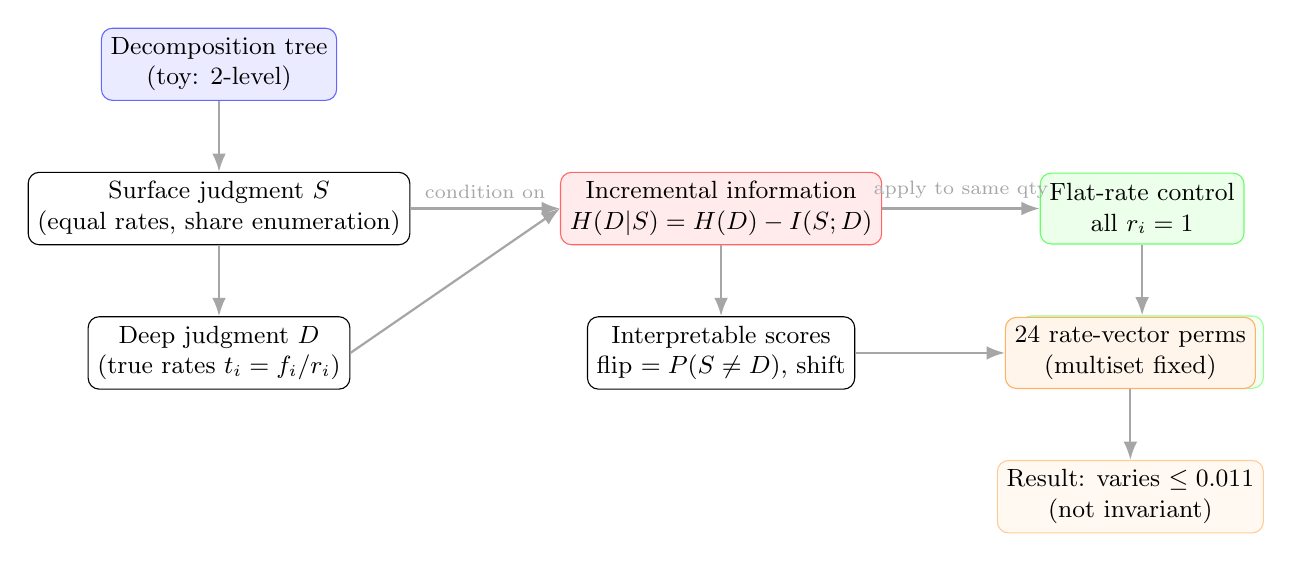
\begin{tikzpicture}[
  node distance=0.9cm and 1.1cm,
  box/.style={draw, rounded corners, align=center, minimum height=0.9cm, font=\small},
  lbl/.style={font=\scriptsize},
  arr/.style={->, >=Latex, thick, gray!70}
]
% Left column: decomposition tree
\node[box, draw=blue!60, fill=blue!8] (root) {Decomposition tree\\(toy: 2-level)};
\node[box, below=of root] (s) {Surface judgment $S$\\(equal rates, share enumeration)};
\node[box, below=of s] (d) {Deep judgment $D$\\(true rates $t_i=f_i/r_i$)};

% Middle column: quantities
\node[box, right=1.9cm of s, draw=red!60, fill=red!8] (inc) {Incremental information\\$H(D|S)=H(D)-I(S;D)$};
\node[box, below=of inc] (score) {Interpretable scores\\flip $=P(S\neq D)$, shift};

% Right column: controls
\node[box, right=2.0cm of inc, draw=green!60, fill=green!8] (flat) {Flat-rate control\\all $r_i=1$};
\node[box, below=of flat, draw=green!40, fill=green!5] (zero) {Result:\\$H(D|S)=0$ exactly};
\node[box, right=1.9cm of score, draw=orange!60, fill=orange!8] (perm) {24 rate-vector perms\\(multiset fixed)};
\node[box, below=of perm, draw=orange!40, fill=orange!5] (inv) {Result: varies $\leq 0.011$\\(not invariant)};

\draw[arr] (root) -- (s);
\draw[arr] (s) -- (d);
\draw[arr] (s.east) -- node[lbl, above] {condition on} (inc.west);
\draw[arr] (d.east) -- (inc.west);
\draw[arr] (inc) -- (score);
\draw[arr] (inc.east) -- node[lbl, above] {apply to same qty} (flat.west);
\draw[arr] (flat) -- (zero);
\draw[arr] (score.east) -- (perm.west);
\draw[arr] (perm) -- (inv);
\end{tikzpicture}
\caption{Scoring protocol: decomposition tree $\rightarrow$ conditional information increment $\rightarrow$ two negative controls. Left column: the toy 2-level structure. Middle column: the precomputable scoring quantities. Right column: the flat-rate control (exact zero by algebraic identity) and the 24-permutation sensitivity check (variation $\leq 0.011$, not invariance). The flat-rate control serves as a unit test of the implementation, not as an empirical control.}
\label{fig:scoring-protocol}
\end{figure}
 in the English paper
% Dependencies: \usepackage{tikz}, \usetikzlibrary{positioning,arrows.meta,calc}
\begin{figure}[t]
\centering
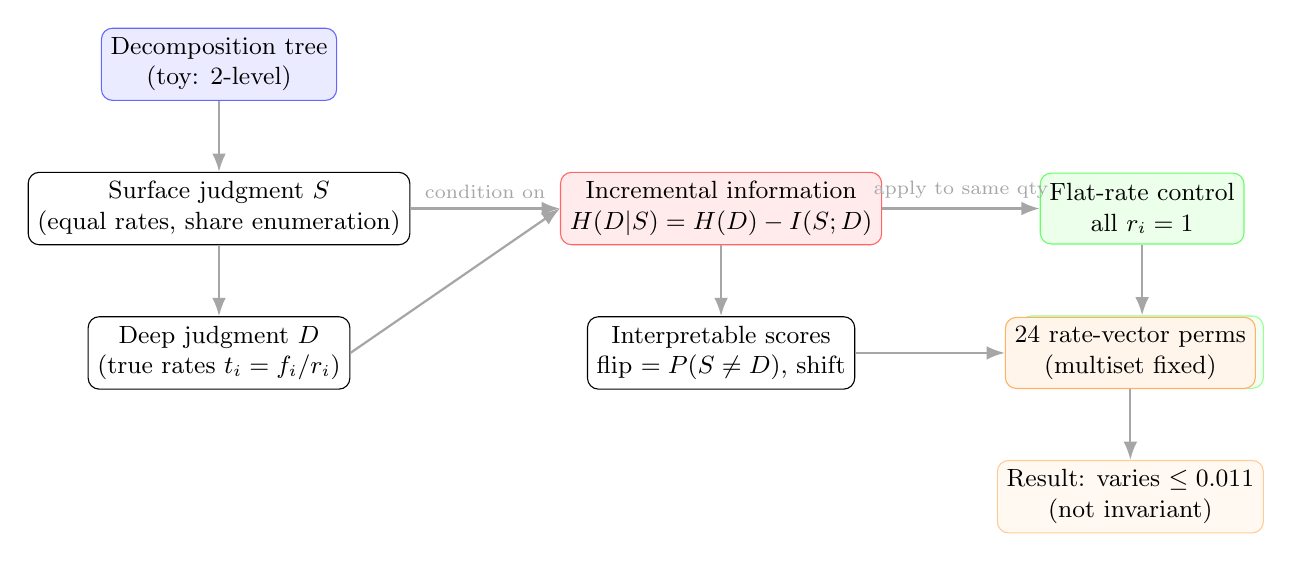
\begin{tikzpicture}[
  node distance=0.9cm and 1.1cm,
  box/.style={draw, rounded corners, align=center, minimum height=0.9cm, font=\small},
  lbl/.style={font=\scriptsize},
  arr/.style={->, >=Latex, thick, gray!70}
]
% Left column: decomposition tree
\node[box, draw=blue!60, fill=blue!8] (root) {Decomposition tree\\(toy: 2-level)};
\node[box, below=of root] (s) {Surface judgment $S$\\(equal rates, share enumeration)};
\node[box, below=of s] (d) {Deep judgment $D$\\(true rates $t_i=f_i/r_i$)};

% Middle column: quantities
\node[box, right=1.9cm of s, draw=red!60, fill=red!8] (inc) {Incremental information\\$H(D|S)=H(D)-I(S;D)$};
\node[box, below=of inc] (score) {Interpretable scores\\flip $=P(S\neq D)$, shift};

% Right column: controls
\node[box, right=2.0cm of inc, draw=green!60, fill=green!8] (flat) {Flat-rate control\\all $r_i=1$};
\node[box, below=of flat, draw=green!40, fill=green!5] (zero) {Result:\\$H(D|S)=0$ exactly};
\node[box, right=1.9cm of score, draw=orange!60, fill=orange!8] (perm) {24 rate-vector perms\\(multiset fixed)};
\node[box, below=of perm, draw=orange!40, fill=orange!5] (inv) {Result: varies $\leq 0.011$\\(not invariant)};

\draw[arr] (root) -- (s);
\draw[arr] (s) -- (d);
\draw[arr] (s.east) -- node[lbl, above] {condition on} (inc.west);
\draw[arr] (d.east) -- (inc.west);
\draw[arr] (inc) -- (score);
\draw[arr] (inc.east) -- node[lbl, above] {apply to same qty} (flat.west);
\draw[arr] (flat) -- (zero);
\draw[arr] (score.east) -- (perm.west);
\draw[arr] (perm) -- (inv);
\end{tikzpicture}
\caption{Scoring protocol: decomposition tree $\rightarrow$ conditional information increment $\rightarrow$ two negative controls. Left column: the toy 2-level structure. Middle column: the precomputable scoring quantities. Right column: the flat-rate control (exact zero by algebraic identity) and the 24-permutation sensitivity check (variation $\leq 0.011$, not invariance). The flat-rate control serves as a unit test of the implementation, not as an empirical control.}
\label{fig:scoring-protocol}
\end{figure}
 in the English paper
% Dependencies: \usepackage{tikz}, \usetikzlibrary{positioning,arrows.meta,calc}
\begin{figure}[t]
\centering
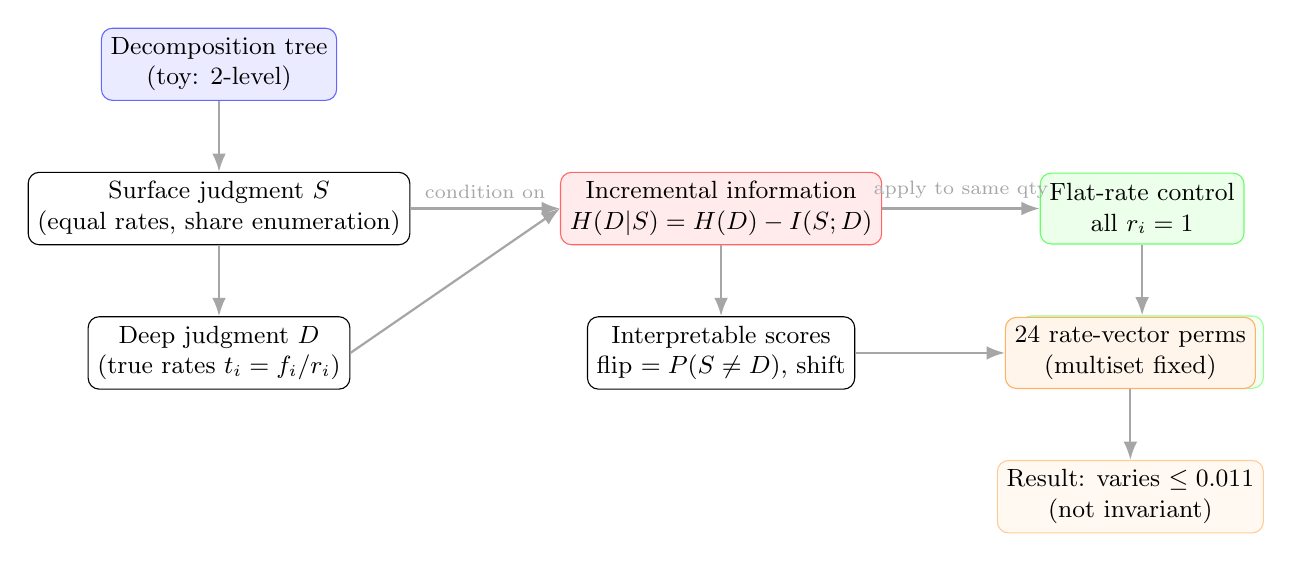
\begin{tikzpicture}[
  node distance=0.9cm and 1.1cm,
  box/.style={draw, rounded corners, align=center, minimum height=0.9cm, font=\small},
  lbl/.style={font=\scriptsize},
  arr/.style={->, >=Latex, thick, gray!70}
]
% Left column: decomposition tree
\node[box, draw=blue!60, fill=blue!8] (root) {Decomposition tree\\(toy: 2-level)};
\node[box, below=of root] (s) {Surface judgment $S$\\(equal rates, share enumeration)};
\node[box, below=of s] (d) {Deep judgment $D$\\(true rates $t_i=f_i/r_i$)};

% Middle column: quantities
\node[box, right=1.9cm of s, draw=red!60, fill=red!8] (inc) {Incremental information\\$H(D|S)=H(D)-I(S;D)$};
\node[box, below=of inc] (score) {Interpretable scores\\flip $=P(S\neq D)$, shift};

% Right column: controls
\node[box, right=2.0cm of inc, draw=green!60, fill=green!8] (flat) {Flat-rate control\\all $r_i=1$};
\node[box, below=of flat, draw=green!40, fill=green!5] (zero) {Result:\\$H(D|S)=0$ exactly};
\node[box, right=1.9cm of score, draw=orange!60, fill=orange!8] (perm) {24 rate-vector perms\\(multiset fixed)};
\node[box, below=of perm, draw=orange!40, fill=orange!5] (inv) {Result: varies $\leq 0.011$\\(not invariant)};

\draw[arr] (root) -- (s);
\draw[arr] (s) -- (d);
\draw[arr] (s.east) -- node[lbl, above] {condition on} (inc.west);
\draw[arr] (d.east) -- (inc.west);
\draw[arr] (inc) -- (score);
\draw[arr] (inc.east) -- node[lbl, above] {apply to same qty} (flat.west);
\draw[arr] (flat) -- (zero);
\draw[arr] (score.east) -- (perm.west);
\draw[arr] (perm) -- (inv);
\end{tikzpicture}
\caption{Scoring protocol: decomposition tree $\rightarrow$ conditional information increment $\rightarrow$ two negative controls. Left column: the toy 2-level structure. Middle column: the precomputable scoring quantities. Right column: the flat-rate control (exact zero by algebraic identity) and the 24-permutation sensitivity check (variation $\leq 0.011$, not invariance). The flat-rate control serves as a unit test of the implementation, not as an empirical control.}
\label{fig:scoring-protocol}
\end{figure}


\section{2. Model}\label{model}

A workload has four components with shares $f_i$ sampled from $\mathrm{Dirichlet}(1,1,1,1)$. Each component has a rate $\mathrm{rate}_i$.

\begin{itemize}
\tightlist
\item
  Surface judgment $S$: assume all $\mathrm{rate}_i=1$, so time share $\propto f_i$, bottleneck $=\arg\max_i f_i$.
\item
  Deep judgment $D$: apply true rates, $t_i=f_i/\mathrm{rate}_i$ \citep{rooflineTime2020}, bottleneck $=\arg\max_i t_i$.
\end{itemize}

Incremental quantities:

\[
\text{flip}=P(S\neq D),\qquad \text{shift}=\mathbb{E}\,|\mathrm{share}_D-\mathrm{share}_S|,
\] \[
H(D|S)=H(D)-I(S;D).
\]

Four platforms: RTX 5090 (max/min rate ratio 51.9), Thor T5000 (9.9), RTX 4090 (287.4), A100 (44.3).

\section{3. Results}\label{results}

\begin{longtable}[]{@{}llll@{}}
\toprule\noalign{}
Platform & flip & shift & $H(D|S)$ (bits) \\
\midrule\noalign{}
\endhead
\bottomrule\noalign{}
\endlastfoot
RTX 5090 & 0.527 & 0.200 & 0.76 \\
Thor T5000 & 0.434 & 0.166 & 0.71 \\
RTX 4090 & 0.563 & 0.231 & 0.77 \\
A100 & 0.556 & 0.218 & 0.74 \\
\end{longtable}

Three hand-derived anchors reproduce exactly: T5000 50/50 → 80\%; T5000 70/30 → 63\%; 5090 scalar 40\% with issue rate halved → 40\% slower.

The correction is not monotone in rate-ratio \emph{extremity}: A100 (ratio 44.3) exceeds 5090 (ratio 51.9) in shift. We therefore claim only dependence on rate-ratio \emph{structure}; with four platforms this is a 4-point structural observation, not a scaling law.

\section{4. Negative controls and defenses}\label{negative-controls-and-defenses}

\textbf{(1) Flat-rate control --- measured arm.} Set all rates of a placeholder hardware to 1. Result: flip = 0.0000, shift = 0.0000, $H(D|S)=0.0$ --- \textbf{exactly} zero, not merely small. This rules out ``deep merely forwards surface information.''

\textbf{(2) Parameter--depth permutation --- measured arm.} Permute the rate vector across the four components in all 24 ways, holding the multiset fixed. If the increment tracked the \emph{label} of which component is called deep, it would change; if it tracks rate-ratio \emph{content}, it should not. Result: identity permutation reproduces the main numbers exactly; across permutations flip varies only within a narrow Monte-Carlo band (5090: 0.5251--0.5304). The criterion is de-depth-ified.

\textbf{(3) Intra-level type control --- design-level argument.} In our two-level model, surface is enumeration-type and deep is judgment-type, differing only in the rate vector: type is not confounded with depth. An earlier node-level model did confound them, and there the type control ran \emph{against} the hypothesis (enumeration 0.5841 bits \textgreater{} judgment 0.1344 bits). That number comes from a different, confounded model and is not used as evidence.

\textbf{HARKing declaration.} All criteria, formulas, and the make-or-break test (deep-only information \textgreater{} 0 on real platforms, = 0 on the flat control) were committed before data generation (commit \texttt{eb1b0598c}, 17:39, preceding \texttt{718394ece}, 18:06). The only post hoc change \emph{weakened} a secondary hypothesis (monotonicity in extremity → dependence on structure) because the data contradicted the stronger form.

\section{5. Tree demonstration (a 4-point observation)}\label{tree-demonstration-a-4-point-observation}

Under a two-way split (compute vs memory), the correction decomposes into branch-level and within-branch components whose four cells sum to 1 (additive self-consistency):

\begin{longtable}[]{@{}
  >{\raggedright\arraybackslash}p{(\linewidth - 10\tabcolsep) * \real{0.1667}}
  >{\raggedright\arraybackslash}p{(\linewidth - 10\tabcolsep) * \real{0.1667}}
  >{\raggedright\arraybackslash}p{(\linewidth - 10\tabcolsep) * \real{0.1667}}
  >{\raggedright\arraybackslash}p{(\linewidth - 10\tabcolsep) * \real{0.1667}}
  >{\raggedright\arraybackslash}p{(\linewidth - 10\tabcolsep) * \real{0.1667}}
  >{\raggedright\arraybackslash}p{(\linewidth - 10\tabcolsep) * \real{0.1667}}@{}}
\toprule\noalign{}
\begin{minipage}[b]{\linewidth}\raggedright
Platform
\end{minipage} & \begin{minipage}[b]{\linewidth}\raggedright
co-flip
\end{minipage} & \begin{minipage}[b]{\linewidth}\raggedright
within-flip
\end{minipage} & \begin{minipage}[b]{\linewidth}\raggedright
co-correct
\end{minipage} & \begin{minipage}[b]{\linewidth}\raggedright
within-correct
\end{minipage} & \begin{minipage}[b]{\linewidth}\raggedright
dominant
\end{minipage} \\
\midrule\noalign{}
\endhead
\bottomrule\noalign{}
\endlastfoot
T5000 (9.9) & 0.530 & 0.145 & 0.036 & 0.290 & within \\
A100 (44.3) & 0.399 & 0.442 & 0.045 & 0.114 & branch \\
5090 (51.9) & 0.409 & 0.335 & 0.064 & 0.191 & branch \\
4090 (287.4) & 0.394 & 0.451 & 0.044 & 0.112 & branch \\
\end{longtable}

Segment-level flip reproduces the 1D main result exactly. The mildest platform (T5000) is within-branch dominant; the three extreme platforms are branch dominant and cluster internally. This is a 4-point structural observation, not a continuous trade-off curve; the split is fixed to compute/memory and alternatives are untested; the extension is post hoc and unregistered but inherits the preregistered flat control.

\section{6. Scope, differentiation, and extension space}\label{scope-differentiation-and-extension-space}

\textbf{A scoring basis, not a solution.} What we deliver is a protocol for how to compute and falsify a node's information increment. It does not solve reward hacking, recover a true objective, or validate any objective-expansion mechanism.

\textbf{Differentiation.} Information gain, roofline, and PID are established tools. Specification Self-Correction (Gallego 2025, arXiv:2507.18742) performs test-time natural-language critique and rewrite of a specification, using no information gain, tree structure, conditional entropy, or quantitative scoring, and no weight updates. Our relation to it is \emph{upstream}: we provide the measurable basis for scoring nodes, and do not touch specification revision.

\begin{longtable}[]{@{}
  >{\raggedright\arraybackslash}p{(\linewidth - 12\tabcolsep) * \real{0.1429}}
  >{\raggedright\arraybackslash}p{(\linewidth - 12\tabcolsep) * \real{0.1429}}
  >{\raggedright\arraybackslash}p{(\linewidth - 12\tabcolsep) * \real{0.1429}}
  >{\raggedright\arraybackslash}p{(\linewidth - 12\tabcolsep) * \real{0.1429}}
  >{\raggedright\arraybackslash}p{(\linewidth - 12\tabcolsep) * \real{0.1429}}
  >{\raggedright\arraybackslash}p{(\linewidth - 12\tabcolsep) * \real{0.1429}}
  >{\raggedright\arraybackslash}p{(\linewidth - 12\tabcolsep) * \real{0.1429}}@{}}
\toprule\noalign{}
\begin{minipage}[b]{\linewidth}\raggedright
Work
\end{minipage} & \begin{minipage}[b]{\linewidth}\raggedright
Input
\end{minipage} & \begin{minipage}[b]{\linewidth}\raggedright
Output
\end{minipage} & \begin{minipage}[b]{\linewidth}\raggedright
Closed-form
\end{minipage} & \begin{minipage}[b]{\linewidth}\raggedright
Exact-zero control
\end{minipage} & \begin{minipage}[b]{\linewidth}\raggedright
Preregistered
\end{minipage} & \begin{minipage}[b]{\linewidth}\raggedright
Spec revision
\end{minipage} \\
\midrule\noalign{}
\endhead
\bottomrule\noalign{}
\endlastfoot
ID3 information gain & data distribution & split attribute & No (needs data) & No & No & No \\
Roofline \citep{roofline2009} & compute/bandwidth spec & bottleneck regime & Yes & No & No & No \\
PID (Williams \& Beer) & multi-source distribution & unique/redundant/synergistic & No (needs distribution) & No & No & No \\
SSC (2507.18742) & rubric + output & rewritten specification & No (test-time generation) & No & No & \textbf{Yes} \\
This work & hardware spec + prior & node increment $H(D|S)$ & \textbf{Yes} & \textbf{Yes (=0)} & \textbf{Yes} & No (upstream) \\
\end{longtable}

The table delineates rather than prioritizes: we do not replicate any existing row. We supply one uncovered cell --- that a node's information increment is closed-form computable and falsifiable by an exact-zero control.

\textbf{Extension space (not implemented).} The tree here is the simplest example structure. Richer versions could introduce Bayesian updating from new data, multiple assumption constraints, and structure selection under a minimum-description-length criterion. None of these is implemented or claimed here; we only state the boundary of extensibility.

\section{7. Limitations}\label{limitations}

\begin{itemize}
\tightlist
\item
  Flip rate and share shift are \textbf{interpretable scores}, not mutual information; the strict quantity is $H(D|S)$.
\item
  The 4090 and A100 lack native FP4; their FP4 rates use a $0.5\times$ FP16 proxy, so the 4090's extreme ratio is partly a proxy artifact.
\item
  The workload prior is uniform Dirichlet and does not model real low-precision-heavy LLM inference; the flat-control zeroing and structural observation are prior-robust by construction, while absolute flip rates would shift under a biased prior.
\item
  Monotonicity fails (A100 \textgreater{} 5090 in shift); four platforms cannot support a scaling law.
\item
  The tree extension is post hoc, 4-point, and fixed-split; the intra-level type control is a design-level argument, not a measured arm.
\item
  Single domain: all four platforms are GPUs, anchors are hand-derived, no measured trace is used. External spot-checking on public data is future work.
\end{itemize}

\section{8. Conclusion}\label{conclusion}

We demonstrate a closed-form, negative-controlled, preregistrable protocol for scoring decomposition-tree nodes. In the toy domain of GPU bottleneck diagnosis, the surface judgment is wrong 43--56\% of the time; the deep increment is 0.17--0.23 in time-share shift and 0.71--0.77 bits of deep-only information, and it vanishes exactly under the flat control. The conclusion is limited to the computability and falsifiability of this scoring basis in this domain: it is computable, reproducible, and falsifiable by its own negative control. It claims neither universality nor a solution to any alignment problem.

\begin{center}\rule{0.5\linewidth}{0.5pt}\end{center}


\bibliography{../submission-staging/references}
\bibliographystyle{tmlr}

\end{document}
